% Author: Izaak Neutelings (September 2021)
% Inspiration:
%   https://www.asimovinstitute.org/neural-network-zoo/
%   https://www.youtube.com/watch?v=aircAruvnKk&list=PLZHQObOWTQDNU6R1_67000Dx_ZCJB-3pi&index=1
\documentclass[border=3pt,tikz]{standalone}
\usepackage{amsmath} % for aligned
\usepackage{listofitems} % for \readlist to create arrays
\usetikzlibrary{arrows.meta} % for arrow size
\usepackage[outline]{contour} % glow around text
\contourlength{1.4pt}

\tikzset{>=latex} % for LaTeX arrow head

% COLORS
\usepackage{xcolor}
\colorlet{myred}{red!80!black}
\colorlet{myblue}{blue!80!black}
\colorlet{mygreen}{green!60!black}
\colorlet{myorange}{orange!70!red!60!black}
\colorlet{mydarkred}{red!30!black}
\colorlet{mydarkblue}{blue!40!black}
\colorlet{mydarkgreen}{green!30!black}

% STYLES
\tikzset{
    >=latex, % for default LaTeX arrow head
    node/.style={thick,circle,draw=myblue,minimum size=22,inner sep=0.5,outer sep=0.6},
    node in/.style={node,green!20!black,draw=mygreen!30!black,fill=mygreen!25},
    node hidden/.style={node,blue!20!black,draw=myblue!30!black,fill=myblue!20},
    node convol/.style={node,orange!20!black,draw=myorange!30!black,fill=myorange!20},
    node out/.style={node,red!20!black,draw=myred!30!black,fill=myred!20},
    connect/.style={thick,mydarkblue}, %,line cap=round
    connect arrow/.style={-{Latex[length=4,width=3.5]},thick,mydarkblue,shorten <=0.5,shorten >=1},
    node 1/.style={node in}, % node styles, numbered for easy mapping with \nstyle
    node 2/.style={node hidden},
    node 3/.style={node out}
}
\def\nstyle{int(\lay<\Nnodlen?min(2,\lay):3)} % map layer number onto 1, 2, or 3

\begin{document}


% NEURAL NETWORK activation
% https://www.youtube.com/watch?v=aircAruvnKk&list=PLZHQObOWTQDNU6R1_67000Dx_ZCJB-3pi&index=1
    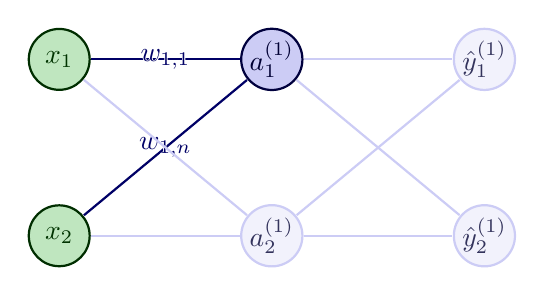
\begin{tikzpicture}[x=2.7cm,y=1.6cm]
        \message{^^JNeural network activation}
        \def\NI{2} % number of nodes in input layer
        \def\NH{2} % number of nodes in hidden layer
        \def\NO{2} % number of nodes in output layer
        \def\yshift{0.4} % shift last node for dots

        % INPUT LAYER
        \foreach \i [evaluate={\c=int(\i==\NI); \y=\NI/2-\i-\c*\yshift; \index=(int(\i));}]
        in {1,...,\NI}{ % loop over nodes
            \node[node in,outer sep=0.6] (NI-\i) at (0,\y) {$x_{\index}$};
        }

        % Hidden Layer
        \foreach \i [evaluate={\c=int(\i==\NH); \y=\NH/2-\i-\c*\yshift; \index=(int(\i));}]
        in {1,\NH}{ % loop over nodes
            \ifnum\i=1 % high-lighted node
            \node[node hidden]
            (NH-\i) at (1,\y) {$a_{\index}^{(1)}$};
            \foreach \j [evaluate={\index=(\j<\NI?int(\j):"n");}] in {1,...,\NI}{ % loop over nodes in previous layer
                \draw[connect,white,line width=1.2] (NI-\j) -- (NH-\i);
                \draw[connect] (NI-\j) -- (NH-\i)
                node[pos=0.50] {\contour{white}{$w_{1,\index}$}};
            }
            \else % other light-colored nodes
            \node[node,blue!20!black!80,draw=myblue!20,fill=myblue!5]
            (NH-\i) at (1,\y) {$a_{\index}^{(1)}$};
            \foreach \j in {1,...,\NI}{ % loop over nodes in previous layer
                %\draw[connect,white,line width=1.2] (NI-\j) -- (NO-\i);
                \draw[connect,myblue!20] (NI-\j) -- (NH-\i);
            }
            \fi
        }

        % Output Layer
        \foreach \i [evaluate={\c=int(\i==\NH); \y=\NH/2-\i-\c*\yshift; \index=(int(\i));}]
        in {1,\NO}{ % loop over nodes

            \node[node,blue!20!black!80,draw=myblue!20,fill=myblue!5]
            (NO-\i) at (2,\y) {$\hat{y}_{\index}^{(1)}$};
            \foreach \j in {1,...,\NH}{ % loop over nodes in previous layer
                %\draw[connect,white,line width=1.2] (NI-\j) -- (NO-\i);
                \draw[connect,myblue!20] (NH-\j) -- (NO-\i);
            }
        }

        % DOTS
%  \path (NI-\NI) --++ (0,1+\yshift) node[midway,scale=1.2] {$\vdots$};
    \end{tikzpicture}


\end{document}